\section{The Hypercube Placement Protocol}
\subsection{Services}
\begin{itemize}
 \item Store objects
 \item Restore objects
 \item Remove objects
 \item Optionnaly handle metadata
\end{itemize}


\subsection{Specifications}
\begin{minipage}{0.49\textwidth}
    \begin{tabular}{|c|}
      \hline
      Critical\\
      Production\\
      Feature\\ 
      \hline
    \end{tabular}
\end{minipage}
\begin{minipage}{0.49\textwidth}
    \begin{tabular}{|c|c|}
      \hline
      0 & Nothing done\\
      1 & Specification\\
      2 & Algorithm\\
      3 & Implementation\\ 
      4 & Production\\
      \hline
     \end{tabular}
\end{minipage}




\begin{table}[h]
  \centering
  \begin{tabular}{|c|c|c|c|}
    \hline
    Service name & Description & Utility & State \\
    \hline
    Object placement & & Critical & 0 \\
    Object access & & Critical & 0 \\
    Object deletion & & Production & 0\\
    Data replication & & Critical & 0 \\
    Data integrity check & & Critical & 0 \\ %on each transaction
    Node integrity check & & ? & 0 \\
    Failure detection & & Critical & 0 \\
    Node integrity update & & ? & 0 \\
    Load balancing & & Critical & 0 \\
    Data balancing & & Critical & 0 \\
    Node addition & & Critical & 0 \\
    Node deletion & & Critical & 0 \\
    Quota/Permission & & Production & 0 \\
    File versionning & Here or in metadata handling(delta chunking) ??? & ? & ? \\
    \hline
  \end{tabular}
  \caption{}
\end{table}

\subsection{Local Complexity requirements}
In a \textbf{n} nodes system, \textbf{m} number of objects:\\

\begin{table}[h]
  \centering
  \begin{tabular}{|c|c|c|}
  \hline
  Description & Time & Space\\
  \hline
  Object placement & $O(\ln(n))$ &  $O(\ln(n))$ \\
  Object access & $O(\ln(n))$ &  $O(\ln(n))$ \\
  Object deletion & $O(\ln(n))$ & $O(\ln(n))$\\
  Data replication & O(max( object placement, object access)) & O(max( object placement, object access))\\
  Data integrity check & O(1) & O(1) \\
  Load balancing & $O(\ln(n))$ &  $O(\ln(n))$ \\
  Data balancing & $\frac{1}{m}$ migrations & $\frac{1}{m}$ migrations\\ %when a node is over filled
  Node addition & $\frac{1}{m}$ migrations & $\frac{1}{m}$ migrations\\
  Node deletion & $\frac{1}{m}$ migrations & $\frac{1}{m}$ migrations\\
  Node integrity check & ? & ? \\ % we assume node still alive, if not it's node deletion
  Node map(store on a node) & ? & $O(1)$ \\
  Node map update & $O(1)$ & $O(1)$ \\
  Node state & ? & $O(\ln(n))$ \\
  Node state update & $O(\ln(n))$ & ? \\
  \hline
  \end{tabular}
  \caption{}
\end{table}
Doit on décrire les différents sytème de cache ?? Filtre de bloom, cache in memmory 1/3 etc ??

\subsection{Global Complexity}
\begin{table}[h]
  \centering
  \begin{tabular}{|c|c|c|}
  \hline
  Description & Time & Space\\
  \hline
  Object placement & $O(\ln(n))$ messages propagation &  $O(n)$ messages  \\
  Object access & $O(\ln(n))$ messages propagation &  $O(n)$ messages \\
  Object deletion & $O(\ln(n))$ messages propagation &  $O(n)$ messages \\
  Data replication & O(max( object placement, object access)) & O(max( object placement, object access))\\
  Data integrity check & O(1) & O(1) \\
  Load balancing & $O(\ln(n))$ messages propagation &  $O(n)$ messages \\
  Data balancing & $\frac{1}{m}$ migrations & $\frac{1}{m}$ migrations\\ %when a node is over filled
  Node addition & $\frac{1}{m}$ migrations & $\frac{1}{m}$ migrations\\
  Node deletion & $\frac{1}{m}$ migrations & $\frac{1}{m}$ migrations\\
  Node map update & $O(\ln{n})$ messages propagation & $O(n)$ messages\\
  Node state update & $O(\ln{n})$ messages propagation & $O(n)$ messages\\
  \hline
  \end{tabular}
  \caption{}
\end{table}


\section{The Global Node Map}
\

\subsection{Nodes clustering}
  \begin{figure}[h]
    \label{node-clustering}
    \centering
    \scalebox{0.9}{
      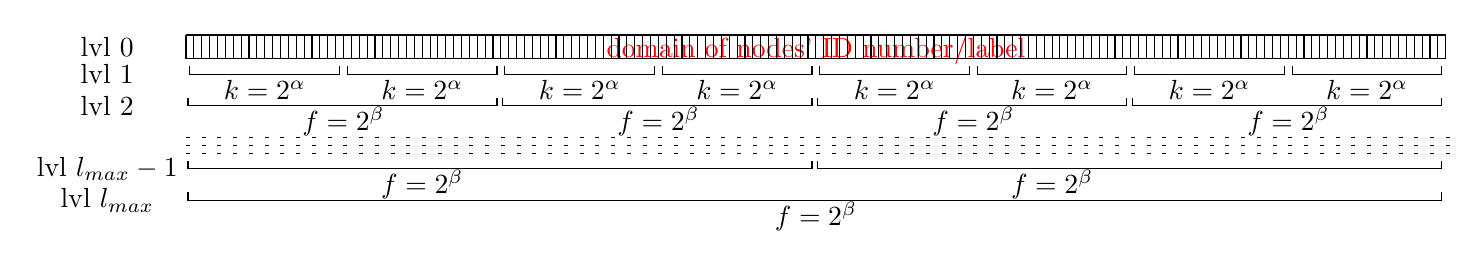
\begin{tikzpicture}

\draw (0,0) -- (16,0) -- (16, -0.3) -- (0, -0.3) -- (0,0);
\node[draw=none, red] at (8, -0.2) {domain of nodes' ID number/label};
\node[draw=none] at (-1, -0.15) {lvl 0};

\foreach \i in {0.1,0.2,...,15.9} {
    \draw (\i,0) -- (\i, -0.3); 
}

\node[draw=none] at (-1, -0.5) {lvl 1};
\foreach \i in {0,2,...,14} {
  \draw (\i + 0.05, -0.4) -- (\i + 0.05, -0.5) -- (\i + 1.95, -0.5) -- (\i + 1.95, -0.4);
  \node[draw=none] at (\i + 1, -0.7) {$k = 2^{\alpha}$};
}

\node[draw=none] at (-1, -0.9) {lvl 2};
\foreach \i in {0,4,8,12} {
  \draw (\i + 0.025, -0.8) -- (\i + 0.025, -0.9) -- (\i + 3.95, -0.9) -- (\i + 3.95, -0.8);
  \node[draw=none] at (\i + 2, -1.1) {$f=2^{\beta}$};
}

\foreach \i in {0,0.2,0.4,...,16} {
  \draw (\i,-1.3) -- (\i+0.05, -1.3) ;
  \draw (\i,-1.4) -- (\i+0.05, -1.4) ;
  \draw (\i,-1.5) -- (\i+0.05, -1.5) ;
}

\node[draw=none] at (-1, -1.7) {lvl $l_{max}-1$};
\foreach \i in {0,8} {
  \draw (\i + 0.025, -1.6) -- (\i + 0.025, -1.7) -- (\i + 7.95, -1.7) -- (\i + 7.95, -1.6);
  \node[draw=none] at (\i + 3, -1.9) {$f=2^{\beta}$};
}

\node[draw=none] at (-1, -2.1) {lvl $l_{max}$};
\draw (0.025, -2) -- (0.025, -2.1) -- (15.95, -2.1) -- (15.95, -2);
\node[draw=none] at (8, -2.3) {$f=2^{\beta}$};

\end{tikzpicture}
    }
    \caption{2-2-hyper cube structure}
  \end{figure}
  
The main idea is to split nodes in \textbf{k}-nodes cluster and to aggregate such cluster in second order cluster and so on( 
in a fractal mod). In this papers we will consider a cluster as an Hyper Cube where vertex are node and edges is connection 
between node( UDP/TCP connections). \\

We split the node-ids domain in buckets of \textbf{k} nodes( that make a cluster) then we split we buckets domain in hight order buckets
of \textbf{f} low order buckets and we repeat. 

\subsection{Global Map}
\begin{minipage}{0.49\textwidth}
   \centering
   \scalebox{0.3}{
       \begin{tikzpicture}
   \node[point] (a) {};
   \node[point, below right=of a] (a1) {};
   \node[node, below right=of a1] (0) {};
   \node[node, right=of 0](1) {};
   \node[node, below=of 1](2) {};
   \node[node, left=of 2] (3) {};
   \draw (3) -- (2) -- (1) -- (0) -- (3);
   
   \node[node, right=of 1] (4) {};
   \node[node, right=of 4] (5) {};
   \node[node, below=of 5] (6) {};
   \node[node, left=of 6] (7) {};
   \draw (7) -- (6) -- (5) -- (4) -- (7);
   \draw[dashed] (1) -- (4);
   \draw[dashed] (2) -- (7);
   
   \node[point, above right=of 5] (b1) {};
   \node[point, right=of b1] (a2) {};
   \node[node, below right=of a2] (8) {};
   \node[node, right=of 8] (9) {};
   \node[node, below=of 9] (10) {};
   \node[node, left=of 10] (11) {};
   \draw (11) -- (10) -- (9) -- (8) -- (11);
   \draw[dashed] (5) -- (8);
   \draw[dashed] (6) -- (11);
   
   \node[node, right=of 9] (12) {};
   \node[node, right=of 12] (13) {};
   \node[node, below=of 13] (14) {};
   \node[node, left=of 14] (15) {};
   \draw (15) -- (14) -- (13) -- (12) -- (15);
   \draw[dashed] (9) -- (12);
   \draw[dashed] (10) -- (15);
   \node[point, above right=of 13] (b2) {};
   \node[point, above right=of b2] (b) {};
   
   %% Deuxième ligne
   \node[node, below=of 3] (16) {};
   \node[node, right=of 16](17) {};
   \node[node, below=of 17](18) {};
   \node[node, left=of 18] (19) {};
   \draw (19) -- (18) -- (17) -- (16) -- (19);
   \node[point, below left=of 19] (d1) {};
   \node[point, below=of d1] (a3) {};
   
   \node[node, right=of 17] (20) {};
   \node[node, right=of 20] (21) {};
   \node[node, below=of 21] (22) {};
   \node[node, left=of 22] (23) {};
   \draw (23) -- (22) -- (21) -- (20) -- (23);
   \draw[dashed] (17) -- (20);
   \draw[dashed] (18) -- (23);
   \draw[dashed] (3) -- (16);
   \draw[dashed] (2) -- (17);
   \draw[dashed] (7) -- (20);
   \draw[dashed] (6) -- (21);
   
   

   \node[node, below=of 11] (24) {};
   \node[node, right=of 24] (25) {};
   \node[node, below=of 25] (26) {};
   \node[node, left=of 26] (27) {};
   \draw (27) -- (26) -- (25) -- (24) -- (27);
   \draw[dashed] (21) -- (24);
   \draw[dashed] (22) -- (27);
   \draw[dashed] (11) -- (24);
   \draw[dashed] (10) -- (25);
   
   \node[node, right=of 25] (28) {};
   \node[node, right=of 28] (29) {};
   \node[node, below=of 29] (30) {};
   \node[node, left=of 30] (31) {};
   \draw (31) -- (30) -- (29) -- (28) -- (31);
   \draw[dashed] (25) -- (28);
   \draw[dashed] (26) -- (31);
   \draw[dashed] (14) -- (29);
   \draw[dashed] (15) -- (28);
   
   \node[point, below right=of 30] (c2) {};
   \node[point, below=of c2] (b4) {};
   \node[point, below right=of 22] (c1) {};
   \node[point, right=of c1] (d2) {};
   
   %%Trosième ligne
   \node[node, below right=of a3] (32) {};
   \node[node, right=of 32](33) {};
   \node[node, below=of 33](34) {};
   \node[node, left=of 34] (35) {};
   \draw (35) -- (34) -- (33) -- (32) -- (35);
   \draw[dashed] (18) -- (33);
   \draw[dashed] (19) -- (32);

   
   \node[node, right=of 33] (36) {};
   \node[node, right=of 36] (37) {};
   \node[node, below=of 37] (38) {};
   \node[node, left=of 38] (39) {};
   \draw (39) -- (38) -- (37) -- (36) -- (39);
   \draw[dashed] (33) -- (36);
   \draw[dashed] (34) -- (39);
   \draw[dashed] (22) -- (37);
   \draw[dashed] (23) -- (36);
   \node[point, above right=of 37] (b3) {};
   \node[point, right=of b3] (a4) {};
   
   

   \node[node, below right=of a4] (40) {};
   \node[node, right=of 40] (41) {};
   \node[node, below=of 41] (42) {};
   \node[node, left=of 42] (43) {};
   \draw (43) -- (42) -- (41) -- (40) -- (43);
   \draw[dashed] (37) -- (40);
   \draw[dashed] (38) -- (43);
   \draw[dashed] (27) -- (40);
   \draw[dashed] (26) -- (41);
   
   \node[node, right=of 41] (44) {};
   \node[node, right=of 44] (45) {};
   \node[node, below=of 45] (46) {};
   \node[node, left=of 46] (47) {};
   \draw (47) -- (46) -- (45) -- (44) -- (47);
   \draw[dashed] (41) -- (44);
   \draw[dashed] (42) -- (47);
   \draw[dashed] (31) -- (44);
   \draw[dashed] (30) -- (45);
   
   %%Quatrième ligne
   \node[node, below=of 35] (48) {};
   \node[node, right=of 48] (49) {};
   \node[node, below=of 49] (50) {};
   \node[node, left=of 50] (51) {};
   \draw (51) -- (50) -- (49) -- (48) -- (51);
   \draw[dashed] (34) -- (49);
   \draw[dashed] (35) -- (48);
   \node[point, below left=of 51] (d3) {};
   \node[point, below left=of d3] (d) {};
   
   \node[node, right=of 49] (52) {};
   \node[node, right=of 52] (53) {};
   \node[node, below=of 53] (54) {};
   \node[node, left=of 54] (55) {};
   \draw (55) -- (54) -- (53) -- (52) -- (55);
   \draw[dashed] (49) -- (52);
   \draw[dashed] (50) -- (55);
   \draw[dashed] (38) -- (53);
   \draw[dashed] (39) -- (52);
   \node[point, below right=of 54] (c3) {};
   \node[point, right=of c3] (d4) {};
   
   
   \node[node, below=of 43] (56) {};
   \node[node, right=of 56] (57) {};
   \node[node, below=of 57] (58) {};
   \node[node, left=of 58] (59) {};
   \draw (59) -- (58) -- (57) -- (56) -- (59);
   \draw[dashed] (43) -- (56);
   \draw[dashed] (42) -- (57);
   \draw[dashed] (53) -- (56);
   \draw[dashed] (54) -- (59);
   
   \node[node, right=of 57] (60) {};
   \node[node, right=of 60] (61) {};
   \node[node, below=of 61] (62) {};
   \node[node, left=of 62] (63) {};
   \draw (63) -- (62) -- (61) -- (60) -- (63);
   \draw[dashed] (57) -- (60);
   \draw[dashed] (58) -- (63);
   \draw[dashed] (47) -- (60);
   \draw[dashed] (46) -- (61);
   
   \node[point, below right=of 62] (c4) {};
   \node[point, below right=of c4] (c) {};
   
   %second order hcube
   \draw[green] (a1) -- (b1) -- (c1) -- (d1) -- (a1);
   \draw[green] (a2) -- (b2) -- (c2) -- (d2) -- (a2);
   \draw[green] (a3) -- (b3) -- (c3) -- (d3) -- (a3);
   \draw[green] (a4) -- (b4) -- (c4) -- (d4) -- (a4);
   \draw[red] (a) -- (b) -- (c) -- (d) -- (a);
  \end{tikzpicture}
  
   }
   \captionof{figure}{2-2-hyper cube structure}
\end{minipage}
\begin{minipage}{0.49\textwidth}
So we can see the network, at any level, as an Hyper Cube where vertices are hypercube(recursively).
\end{minipage}\\\\
\begin{table}[h]
  \centering
  \begin{tabular}{|c|c|c|c|c|}
    \hline
    layer & Description & Number of vertices &  Number of nodes & Dimension\\
    \hline
    0		   	& node & 1 & 1 & 0\\
    1		   	& $\alpha-dim$ hcube(vertices are nodes) & f & $f=2̂^{\alpha}$ & $\alpha$\\
    l		   	& $\alpha-dim$ hcube(vertices are $\alpha-dim$ hcube) & $f$ & $f^{l} = 2^{\alpha l}$  & $\alpha$\\
    \hline
  \end{tabular}
  \caption{}
\end{table}

\begin{definition} Global map\\
  $$\text{Let }G^{f}(n), (f,n) \in \mathbb{N} \times \mathbb{N}^{*}, \text{ a global map where }
  \left\{\begin{array}{ll}
     f = 2^{\alpha} & \text{size of a cluster}\\
     n 	& \text{number of nodes}\\ 
     l(n) &  \text{number of layers of hypercube}\\
    \alpha & \text{ mesh parameter}\\
  \end{array}\right.$$\\
  \begin{tabular}{cc}
    let $G^{f}(n)=_{def} (V^{f}(n),E^{f}(n), Id_{f}) =_{def} (Q^{f}(n), Id^{f})$
  \end{tabular}
\end{definition}



\begin{definition} Let $(f,l) \in \mathbb{N} \times \mathbb{N}^{*}$, $G_{l}^{f} = \left\{ G^{f}(n) |n \in \mathbb{N}, l(n) = l \right\}$\\
\end{definition}

\begin{definition} Let $n \in \mathbb{N}^{*}$, $l \in [|1, l(n)|]$, 
$H_{l+1}^{f}(n) = (V_{l+1}^{f}(n), E_{l+1}^{f}(n), Id_{l+1}^{f})$\\
Where $V_{l+1}^{f}(n) = \left\{V_{0}^{f}(n), ..., V_{f-1}^{f}(n)) \right\} \subset (Q_{l}^{f})^{f} $ and $Id_{l+1}^{f}(V_{i}^{f}(n)	)=i$\\
$\forall v \in V, V_{l}^{f}(v) = V_{i}^{f}(n)$ where $i \in [|0,f-1|]$ such that $v \in V_{i}^{f}(n)$, i is uniq
\end{definition}

\begin{definition} global identifier\\
  Let $(f,n) \in \mathbb{N} \times \mathbb{N}^{*}$, and $v \in V$:\\
      $gid_{G^{f}(n)}(v) = gid_{l(n)}(v) \text{ where } \left\{ 
	\begin{array}{llll}
	 gid_{1}(v) & = & Id_{f}(v) & \\
	 gid_{l+1}(v) & = & Id_{l+1}^{f}(V_{l}^{f}(v)) \times 2^{(l-1)\alpha+\alpha} + gid_{l}(v) & | 0 \leq l \le l(n)\\
	\end{array}\right\}$\\  
\end{definition}

\begin{prop}
Let $(f,n) \in \mathbb{N} \times \mathbb{N}^{*} gid_{G^{f}(n)}(v) =\sum_{l=1}^{l(n)-1} Id_{l}^{f}(V_{l}^{f}(v)) \times 2^{(l-1)\alpha}$
\end{prop}


\begin{definition}[ neighbourhood] Let $(f,n) \in \mathbb{N} \times \mathbb{N}^{*}, i \in Q^{f}(n)$,\\
$N^{f}(i) =_{def}\bigcup_{l=1}^{l(n)}{N_{l}^{f}(v)}$\\
$where \left\{
\begin{array}{lll}
 N_{1}^{f} & = &\{j|j\in Q^{f}(n), d_{ham}(i,j)=1\}\\
 N_{1}^{f} & = &\{j|j\in Q^{f}(n), d_{ham}(i,j)=1\}\\
\end{array}\right\}$

\end{definition}


\begin{prop}
  Let $(f,n) \in \mathbb{N} \times \mathbb{N}^{*}$ then $l(n)-1 < \ln(\frac{|G^{f}(n)|}{f}-f) =_{def} \ln(\frac{n}{f}-f) \leq l(n)$\\ 
\end{prop}

\begin{proof}Let $(f,n) \in \mathbb{N} \times \mathbb{N}^{*}$\\
  \begin{itemize}
   \item Case 1 :   $Layers(G^{f}(n))$ is a perfect tree, hence there is $f^{l(n)}$ leaves(1-cluster)\\
      Moreover there is $\frac{|G^{f}(n)|}{f}=\frac{n}{f}$ 1-cluster(ie leaves by construct)\\
    \begin{tabular}{rcl}
      $f^{l(n)}$ & = & $\frac{n}{f}$ \\
      $l(n)\ln(f)$ & = & $\ln(\frac{n}{f})$\\
      $l(n)$ & = & $\ln(\frac{n}{f}-f)$\\ 
    \end{tabular}
   \item Case 2 :   $G^{f}(n)$ is a complete tree\\
     Therefore 
    \begin{tabular}{lclcl}
      $f^{l(n)-1}$ & $<$ & $\frac{|G^{f}(n)|}{f}$ & $\leq$ & $f^{l(n)}$\\
      $(l(n)-1)\ln(f)$ & $<$ & $\ln(\frac{n}{f})$ & $\leq$ & $l(n)\ln(f)$\\
      $l(n)-1$ & $<$ & $\ln(\frac{n}{f}-f)$ & $\leq$ & $l(n)$\\ 
    \end{tabular}
  \end{itemize}
\end{proof}


 
 
\begin{lemma} \label{lemma-min_connexity}
  Let $(k,f,d) \in \mathbb{N} \times \mathbb{N} \times \mathbb{N}^{*}$, $G^{f}$ is $\min(\ln(k),\ln(f))$-connected
\end{lemma}
 
 \begin{proof}
  
 \end{proof}
 
 \begin{lemma}
  Let blablabla, $\forall l \in [|2,lmax-1|]$, the network composed of l-hcube(ie l-hcube are vertices) is f-connexe.
 \end{lemma}

 \begin{proof}
 same proof ass \ref{lemma-min_connexity}
\end{proof}

\begin{lemma}
 If a node is in cluster at d distance of the fronter then it is $k*f^{d}$ connexe with >d distance of fronter.
 Note that d<=ln(n) (esperance en kf(n/2) ? )
\end{lemma}

\begin{proof}
 todo
\end{proof}

\begin{lemma}
 A node as exactly k+f neightbourgs if it is not in the fronteir and k< <k+f otherwith.
\end{lemma}

\begin{proof}
 Todo
\end{proof}


Lets describe the semantic of the network, vertices are nodes where data is/are? stored, edges is the allowed cmmunication 
channel used for all except data transmition. Indeed as soon as data location is computed both node open a direct channel, the network provide low overhead 
with node discovering, data placement, global node map modifications and in the other hand it provide very fast data transfert by bypassing the topologie of the network.
\\
We will call communication rounds : each $\tau$s (something like 0.1, a parameter) each node send data map modification to its neightbourg and heartbeat

\subsection{Object placement}
\begin{minipage}{0.49\textwidth}
   \centering
   \scalebox{0.1}{
     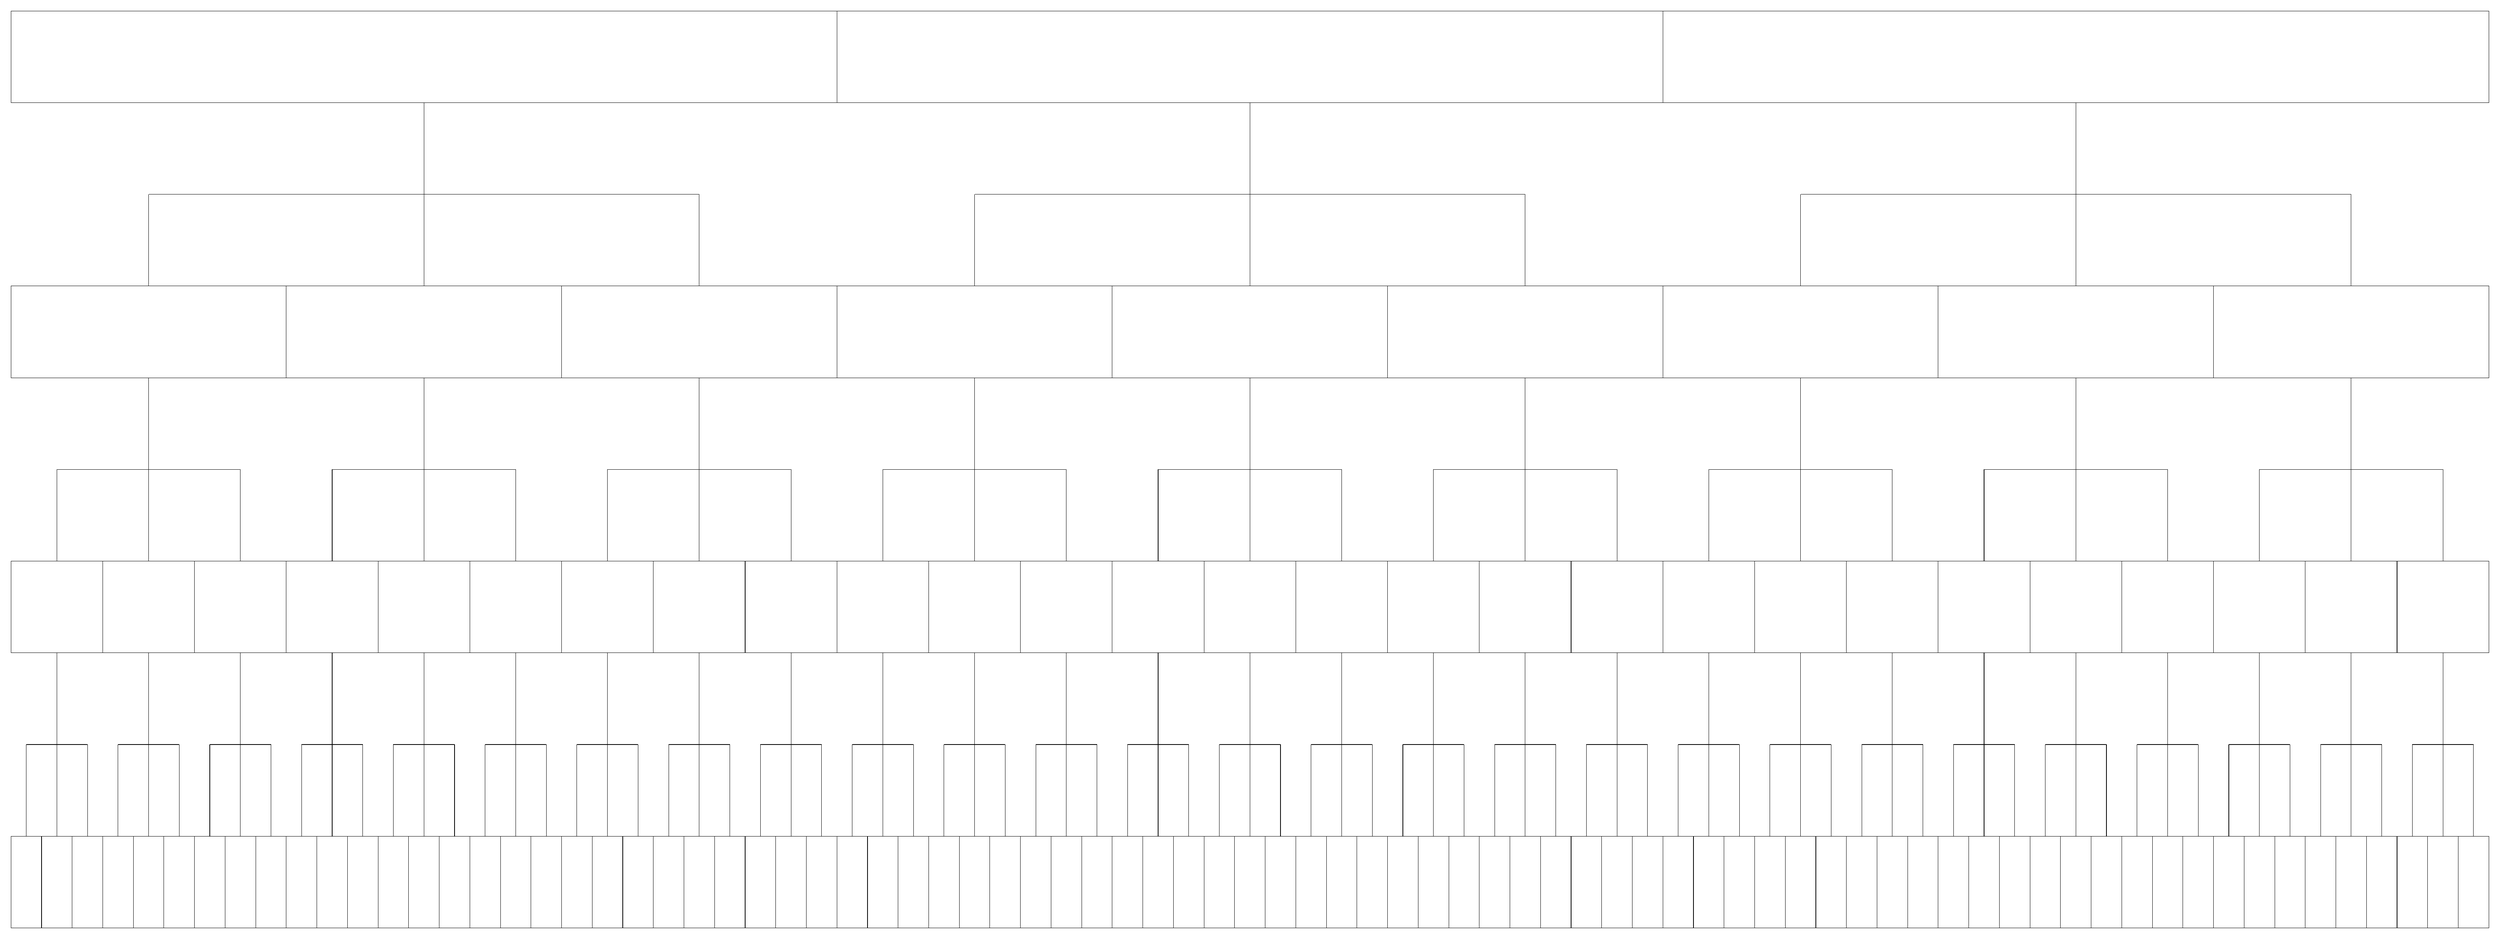
\begin{tikzpicture}
 
% 81 origin
% 27 lvl lmax
% 9 9 9 lvl i
% 3 3 3 lvl 1
% 111  lvl 0
\foreach \r in {3}{%ratio vertical
\foreach \i in {0,1,2} {
    \draw (27 * \i, \r * 0) -- (27 * \i, \r * -1) -- (27 * \i+27, \r * -1) -- (27 * \i+27, \r * 0) -- (27 * \i, \r * 0); 
    \draw (13.5 + 27 * \i, \r * -1) -- (13.5 + 27 * \i, \r * -2);
    \draw (4.5 + 27 * \i, \r * -2) -- (22.5 + 27 * \i, \r * -2);

        
      \foreach \j in {3*\i,3*\i+9,3*\i+18}{
	\draw (9 * \j + 4.5, \r * -2) -- (9 * \j + 4.5, \r * -3);
	\draw (9 * \j, \r * -4) -- (9 * \j, \r * -3) -- (9 * \j+9, \r * -3) -- (9 * \j+9, \r * -4) -- (9 * \j, \r * -4);
	\draw (4.5 + 9 * \j, \r * -4) -- (4.5 + 9 * \j, \r * -5);
        \draw (1.5 + 9 * \j, \r * -5) -- (7.5 + 9 * \j, \r * -5);
        
	\foreach \k in {3*\j,3*\j+3,3*\j+6}{
	  \draw (3 * \k + 1.5, \r * -5) -- (3 * \k + 1.5, \r * -6);
	  \draw (3 * \k, \r * -7) -- (3 * \k, \r * -6) -- (3 * \k+3, \r * -6) -- (3 * \k+3, \r * -7) -- (3 * \k, \r * -7);
	  \draw (1.5 + 3 * \k, \r * -7) -- ( 1.5 + 3 * \k, \r * -8);
	  \draw (0.5 + 3 * \k, \r * -8) -- (2.5 + 3 * \k, \r * -8);
	  
	  \foreach \l in {3*\k,3*\k+1,3*\k+2}{
	    \draw (\l + 0.5, \r * -8) -- (\l + 0.5, \r * -9);
	    \draw (\l, \r * -10) -- (\l, \r * -9) -- (\l+1, \r * -9) -- (\l+1, \r * -10) -- (\l, \r * -10); %faudrait faire des cerlces
% 	    \node[draw=none] at (\l + 0.5, \r * -9.5) {id {\l} };

	  }
	  
	  
	}
    }
}
}
\end{tikzpicture}

   }
   \captionof{figure}{HRW with skeleton, $f=2$, $k=3$}
\end{minipage}
\begin{minipage}{0.49\textwidth}
We will use a distributed version of HRW(ref todo ?) with skeleton. Each lvl of the skeleton will correspond to an hyper cube lvl.\\
Nota bene the skeleton has no need to  be construct and store, indeed we only need(ln(|skeleton|) at each request) so we will rebuild a part each time.
\end{minipage}\\

\begin{algorithmic}
    \State v : noeud précédant
    \State u : noeud courant
    \State s : état de l'agent
    \If {$s = 0$}

    \State $i\gets random(0, deg(u)-1)$
    \State $s \gets deg(u)$
    \State $move\_to( end(v,i) )$
       \Else
    \State $p \gets \min_{ \frac{s}{deg(u)}, 1}$
    \If {$random() \leq p$}
      \State $s \gets 0$
    \Else
      \State $reverse\_move$
    \EndIf
      \EndIf
 \end{algorithmic}

% First lets assumes we have the knowledge of the whole map.\\

\subsection{Adding new node}
Problème du *2, inserer par le bas : deplacement de données??

\subsection{Implementation details}
Memoisation of the entire map if network not to huge : $O(1) message$